% coding:utf-8

\section{Basic Clock Modul +}

\subsection{Übersicht}
\begin{frame}
\frametitle{}
\framesubtitle{}
  \begin{figure}
    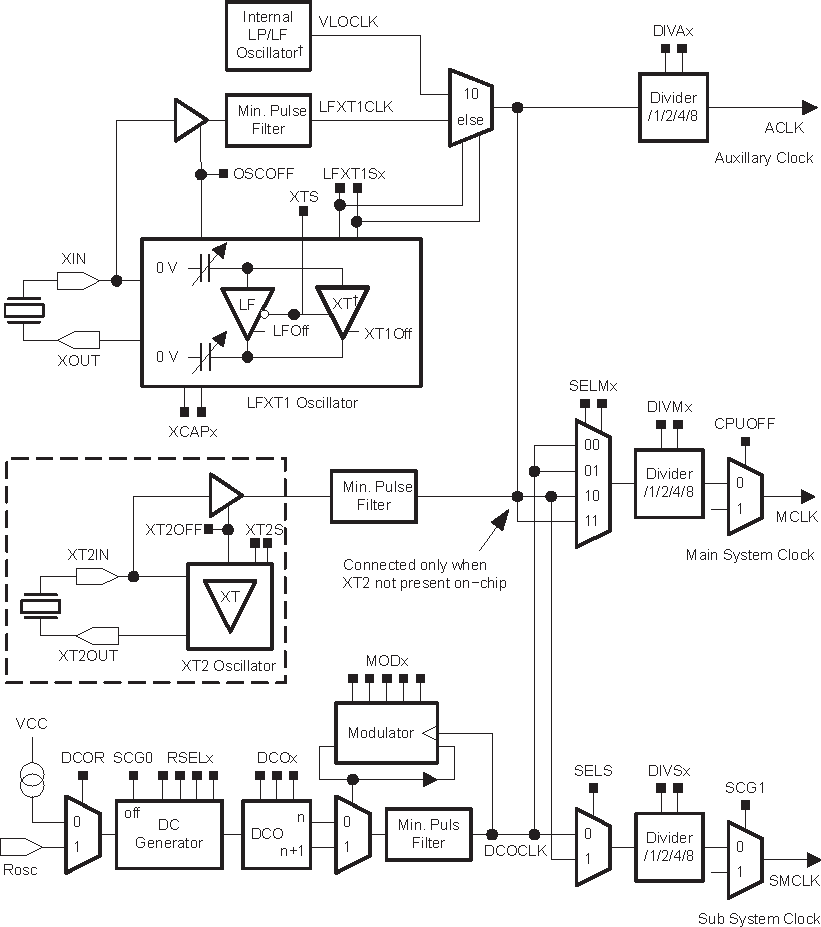
\includegraphics[width=0.5\columnwidth]{fig/ti_fg_bcm_block.pdf}
    \caption{Blockschaltbild}
  \end{figure}
\end{frame}

\begin{frame}
\begin{center}
\tikzstyle{block} = [ draw,fill=blue!20,text width=5em,align=center,
                      rounded corners,minimum height=3em]
\def\radius{.7mm}
\tikzstyle{branch}=[fill,shape=circle,minimum size=3pt,inner sep=0pt]
\begin{tikzpicture}
  \node[block] at (0,4) (lfxt) {LF Quarzosz.};
  \node[block] at (5,4) (aclk) {ACLK};
  \node[block] at (0,2) (xt)   {Quarzosz.};
  \node[block] at (5,2) (mclk) {MCLK};
  \node[block] at (0,0) (dco)  {DCO};
  \node[block] at (5,0) (smclk){SMCLK};
  \uncover<2->{\draw (0,0) node[ellipse,thick,draw=red,minimum height=2cm,
                                minimum width=3cm,draw] {};}
  \draw[-latex] (lfxt.east) -- (aclk.west);
  \draw[-latex] (lfxt.east) -- (mclk.west);
  \draw[-latex,dashed] (lfxt.east) -- (smclk.west);
%   \draw[-latex,dashed] (xt.east) -- (aclk.west);
  \draw[-latex] (xt.east) -- (mclk.west);
  \draw[-latex] (xt.east) -- (smclk.west);
%   \draw[-latex] (dco.east) -- (aclk.west);
  \draw[-latex] (dco.east) -- (mclk.west);
  \draw[-latex] (dco.east) -- (smclk.west);
\end{tikzpicture}
\end{center}
\end{frame}
